\section{Adaptivity}

A regular sparse grid is constructed in a way that takes a cut in diagonal hyperplane, which means
it treats all the dimensions equally. However, there can be an importance difference between the dimensions,
i.e. one dimension might be more important than others. This can be solved by so called dimensional adaptivity.

The most straightforward approach for this type of refinement is adding some
new subspaces in the dimension which function changes rapidly. In order to add a new subspace
\(W_{\vec{l}}\) one should include all the backward neighbours in the current set of subspaces.
This refiment treads all the grid points in one dimension as a uniform way,and called as
dimensionally adaptive refinement. Leads more point in one dimension than other one.

\todok{May be add an example of dimensionally adaptive sparse grid to here.}

Morever, there are some cases exist, where dimensional adaptivity is not to be enough to solve problem.
For instance take a function that is mostly flat, have peaks at certain regions in the domain.
Franke's function is a good example for this~\cite{Franke1979}.

\begin{equation}
    \begin{aligned}
        f(\textbf{x}) & = \frac{3}{4} \exp \left( - \frac{(9x_1-2)^2}{4} - \frac{(9x_2-2)^2}{4} \right) \\
                      & + \frac{3}{4} \exp  \left( - \frac{(9x_1+1)}{49} - \frac{9x_2+1}{10}\right)     \\
                      & + \frac{1}{2} \exp \left( -\frac{(9x_1-7)^2}{4} - \frac{(9x_2-3)^2}{4} \right)  \\
                      & - \frac{1}{5} \exp \left( - (9x_1-4 )^2 -(9x_2-7)\right)
    \end{aligned}
\end{equation}

\begin{figure}
    \centering
    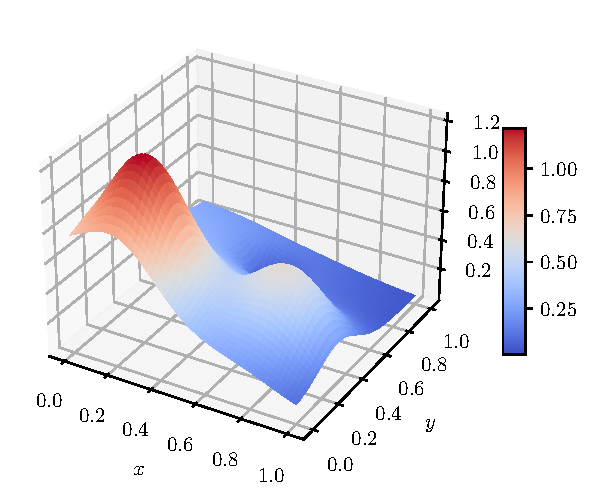
\includegraphics[width=0.4\textwidth]{figures/franke.pdf}
    \caption{Surface plot of Franke's Function.}
    \label{fig:franke}
\end{figure}

A dimensionally adaptive grid would also add more point to regions where the function is mostly flat.
A spatially adaptive grid would overcome this problem. Instead of adding whole incremental grids,
spatial adaption would only include a subset of those points near the region of interest and saves points.

The general approach for spatially adaptive grids is doing the refinement process iteratively.
One could start and initial coarse grid or if knows a grid which is tailored to problem. Using an iterative process
one could simply adds new points (neighboring grid point in the next higher level) to region of interest. To enable usage
of sparse grids algorithms there is also a consistency constraint exist, the grid should contain all the hierarchical
ancestors of all grid points. Figure~\ref{fig:spatialrefiment} shows how this process is done in two-dimensional regular sparse grid.

\begin{figure}
    \centering
    \missingfigure{Add refiment figure here.}
    \caption{Spatial refinement of a selected node in two dimension.}
    \label{fig:spatialrefiment}
\end{figure}